\chapter{Fundamentals of Satellite Constellation
Design}\label{chapter-7-fundamentals-of-satellite-constellation-design}

This chapter establishes the theoretical foundation required to understand the constellation design and analysis that follow. It opens with the observation formalism --- defining how a satellite constellation covers a ground domain and what conditions must hold for a target to be visible to a sensor. It then develops the orbital mechanics principles --- classical orbital elements, the dominant gravitational perturbation, and the resonance condition --- that underpin the Repeating Ground Track Orbit selected for this mission.

\section{Constellation Observation Formalism Introduction}
\label{sec:Constellation_observation_form}
%Improve intro reflection full section
We have previously defined the study domains $\mathcal{D}$ on the Earth's surface. However, for a fire event to be detected, it must fall within the observable coverage domain of the satellite constellation $\mathcal{D_{Cover}}$.  

\subsection{Constellation Definition and State Space}
The satellite constellation is defined as a set of $N$ discrete spacecraft nodes:
\begin{equation}
    \mathcal{C}_{sat} = \{ S_k \}_{k=1}^{N}
\end{equation}
Each satellite $S_k$ is uniquely defined by its \textbf{Orbital State Element} $\vec{A}_k$:
\begin{equation}
    S_{k} \equiv \vec{A}_k
\end{equation}
This vector encapsulates the state-space parameters required to propagate the spacecraft's trajectory. It is composed of the six classical Keplerian orbital elements and a reference epoch, as formally defined in Sec.~\ref{sec:classical_orbital_elements}.


\subsection{Single-Satellite Sensor Visibilty Toward a Ground Target}
This section defines the geometric boundaries and optical constraints that govern the visibility link between a ground target and a spacecraft sensor. The revisit time $t_{rev \to P_j}$ of a satellite $\mathcal{S}_{k}$ over a ground point target $P_{j}$ is fundamentally limited by the geometric constraints of the spacecraft sensor relative to the ground location. To quantify these constraints, such as whether a target is above the local horizon or within the sensor's field of view, we must define a coordinate frame system centered on the observer's location at the ellipsoid surface $\mathcal{E_\oplus}$. The detailed definition of such a local frame, the satellite and ground trajectory, is done in the section. 

\paragraph{Satellite Position Trajectory:}
To analyze the geometry of the sensor-to-target mapping, we first define the trajectories of the spacecraft and the ground targets as time-dependent mappings on the inertial manifold $\mathcal{M}$, as defined in eq. \ref{eq:manifold}. Then, we define the $k$-th satellite $S_k$ as a point mass moving in the inertial frame. Its orbital position with respect to Earth's center of mass $O_{\oplus}$ is defined by the position vector function $\vec{r}_{s,k}$:
\begin{equation}
    \vec{r}_{s,k} : \mathcal{T}_{sim} \to \mathcal{M}, \quad t \mapsto \overrightarrow{r_{s,k}}(t) = \overrightarrow{O_{\oplus}S_{k}}(t)
\end{equation}
\paragraph{Ground Target Trajectory:}
The ground target $P_j$ is fixed to the surface of the WGS84 Reference Ellipsoid $\mathcal{E}_\oplus$. However, due to the Earth's rotation, $P_j$ describes a trajectory in the inertial frame $\mathcal{F}_{J2000}$. We define this motion as the vector function $\vec{r}_j$:
\begin{equation}
    \vec{r}_{j} : \mathcal{T}_{sim} \to \mathcal{M}, \quad t \mapsto \overrightarrow{r_j}(t) = \overrightarrow{O_{\oplus}P_{j}}(t)
\end{equation}
\subsubsection{Topocentric Horizon Coordinate System (SEZ)}
The Topocentric Horizon Coordinate System $\mathcal{F}_{SEZ}$ is the standard frame for defining "look angles" between a ground site and a satellite. We adopt the deffitintion of $\mathcal{F}_{SEZ}$ as done by Vallado\cite{mcclain2001fundamentals}. This frame is also known as $\mathcal{F}_{AltAz}$ because it measures the altitude, also known as elevation $\epsilon$,  and azimuth $\beta$ as shown in Fig. \ref{fig:sez_frame}. This system rotates with the site location $P_{k}$.

\begin{figure}
    \centering
    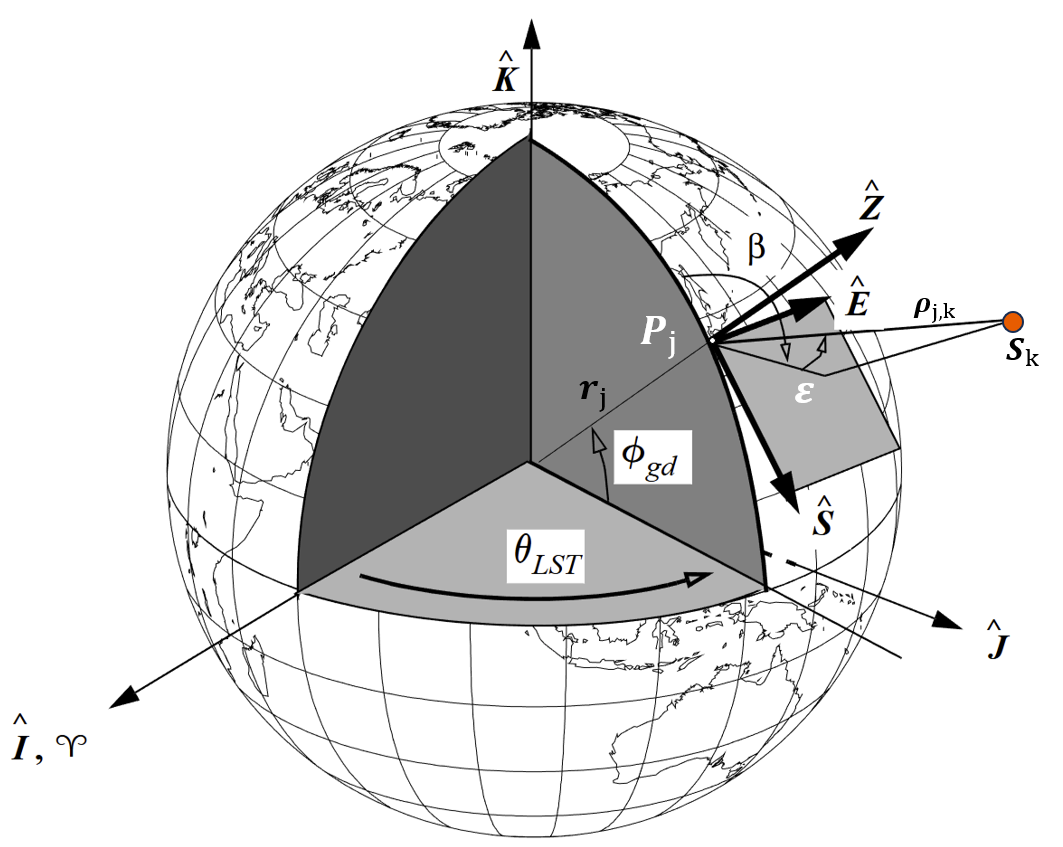
\includegraphics[width=0.5\linewidth]{images/Topocentric_Horizon_Coordinate_System_SEZ.png}
    \caption{\footnotesize{The Topocentric Horizon Coordinate System  $\mathcal{F}_{SEZ}$, "South, East, Zenith frame", or $\mathcal{F}_{AltAz}$. The frame originates at the site location $P_k$ on the Earth's elipsoid $\mathcal{E_\oplus}$. The fundamental plane is the local horizon. The $\hat{S}$ axis points South, the $\hat{E}$ axis points East, and the $\hat{Z}$ axis (Zenith) points radially outward along the local vertical. $\mathcal{F}_{SEZ}$ defines the observation geometry: Azimuth $\beta$ measured clockwise from North, and Elevation $\epsilon$ measured from the horizon plane up to the vector $\rho_{j,k}$ measuring the relative distance between satellite $S_k$ and the ground target $P_j$ .}}
    \label{fig:sez_frame}
\end{figure}
This planetary mobile local frame is is defined by the orthonormal basis $\mathcal{B}_{SEZ} = \{ \hat{\mathbf{s}}, \hat{\mathbf{e}}, \hat{\mathbf{z}} \}$ centered at the target $P_j$, $\mathcal{F}_{SEZ} \equiv  \{ P_{j};\hat{\mathbf{s}}, \hat{\mathbf{e}}, \hat{\mathbf{z}} \}$.  The unit vectors are defined as: $\hat{\boldsymbol{s}}$ (South) along the local meridian, $\hat{\boldsymbol{e}}$ (East) along the local parallel, and $\hat{\boldsymbol{z}}$ (Zenith) along the local vertical

\paragraph{Line-of-Sight (LOS) Vector:}
The relative geometry is governed by the vector connecting the ground target $P_j$ to the satellite $S_k$. We construct this \textbf{Line-of-Sight Vector} $\vec{\rho}_{j,k}$ via the vector subtraction map:
\begin{equation}
    \vec{\rho}_{j,k} : \mathcal{T}_{sim} \to \mathcal{M}, \quad t \mapsto \overrightarrow{\rho_{j,k}}(t) = \overrightarrow{P_{j}S_{k}}(t) = \overrightarrow{r_{s,k}}(t) - \overrightarrow{r_{j}}(t)
\end{equation}

This vector is projected onto the local basis $\mathcal{B}_{SEZ}$ as:
\begin{equation}
    \vec{\rho}_{j,k} = \rho_s \hat{\mathbf{s}} + \rho_e \hat{\mathbf{e}} + \rho_z \hat{\mathbf{z}}
\end{equation}
%%
\paragraph{Relative Position Vector ($\vec{\rho}_{j,k}$):}
The geometry is commanded by the relative displacement between the ground target $P_j$ and the satellite $S_k$. We define the \textbf{Relative Position Vector}  $\vec{\rho}_{j,k}$ via the vector subtraction map:
\begin{equation}
    \vec{\rho}_{j,k} : \mathcal{T}_{sim} \to \mathcal{M}, \quad t \mapsto \vec{\rho}_{j,k}(t) = \overrightarrow{P_{j}S_{k}}(t) = \overrightarrow{r_{s,k}}(t) - \overrightarrow{r_{j}}(t)
\end{equation}
This vector represents the physical distance and direction from the target to the satellite, independent of where the satellite is facing. It is projected onto the local basis $\mathcal{B}_{SEZ}$ as:
\begin{equation}
    \vec{\rho}_{j,k} = \rho_s \hat{\mathbf{s}} + \rho_e \hat{\mathbf{e}} + \rho_z \hat{\mathbf{z}}
\end{equation}
\paragraph{Sensor Boresight Vector ($\hat{\mathbf{b}}_k$):}
Distinct from the relative position, the satellite $S_k$ observation capability depends on its attitude and sensor direction. We define the Sensor Boresight Vector (or Line-of-Sight direction) as the unit vector $\mathbf{b}_{k}$  representing the optical axis of the instrument in the inertial frame:
\begin{equation}
    \hat{\mathbf{b}}_{k} : \mathcal{T}_{sim} \to \mathcal{M}, \quad t \mapsto \hat{\mathbf{b}}_{k}(t) = \mathbf{A}(t) \cdot \hat{\mathbf{b}}_{body}
\end{equation}
where, for $S_k$, $\mathbf{A}(t)$ is the attitude rotation matrix and $\hat{\mathbf{b}}_{body}$ is the fixed sensor axis in the satellite body frame.

\paragraph{Look Angles Definition:}
From these components, we define the look angles as the mapping $\Lambda_{look}: \mathbb{R}^3 \to \mathbb{R}^2$:

\begin{enumerate}
    \item \textbf{Elevation ($\varepsilon$):} The angular height above the local horizon plane. It is derived from the angle between the local zenith $\hat{\mathbf{z}}$ (aligned with $\hat{\boldsymbol{r}}_{j}$ for a spherical approximation) and the relative vector:    \begin{equation}
        \epsilon_{k,j} = \sin^{-1}\left( \frac{\vec{\rho}_{j,k} \cdot \hat{\mathbf{z}}}{\| \vec{\rho}_{j,k} \|} \right), \quad \varepsilon \in \left[ -\frac{\pi}{2}, \frac{\pi}{2} \right]
    \end{equation}
    A positive elevation ($\varepsilon > 0$) indicates that the satellite is above the local geometric horizon and may be able to observe $P_j$, depending on the spacecraft's sensor field of view, line-of-sight orientation, and atmospheric transmission. 
    \item \textbf{Azimuth ($\beta$):} The orientation angle measured clockwise from North ($-\hat{\mathbf{s}}$) to the projection of the satellite vector on the horizon plane.
\begin{equation}
        \beta_{k,j} = \operatorname{atan2}(\rho_e, -\rho_s), \quad \beta \in [0, 2\pi)
    \end{equation}
    where $\operatorname{atan2}(y, x)$ is the multi-valued inverse tangent function used to resolve quadrant ambiguity.
\end{enumerate}

\section{Observational Access}
\label{sec:observational_access}
To formally characterize the observation geometry, we adapt the constellation observation visibility framework established by Lee et al. \cite{lee_satellite_2020}. We introduced the sensor constraints as a condition for visibility.
For a valid observation to occur, the geometric link must satisfy constraints from two distinct reference frames: the target's local horizon (Ground Segment) and the satellite's instrument orientation (Space Segment). As illustrated in Figure \ref{fig:access_window_configs}, visibility is only achieved when the Line-of-Sight (LOS) vector falls within the intersection of these two independent access volumes.

\begin{figure}
    \centering
    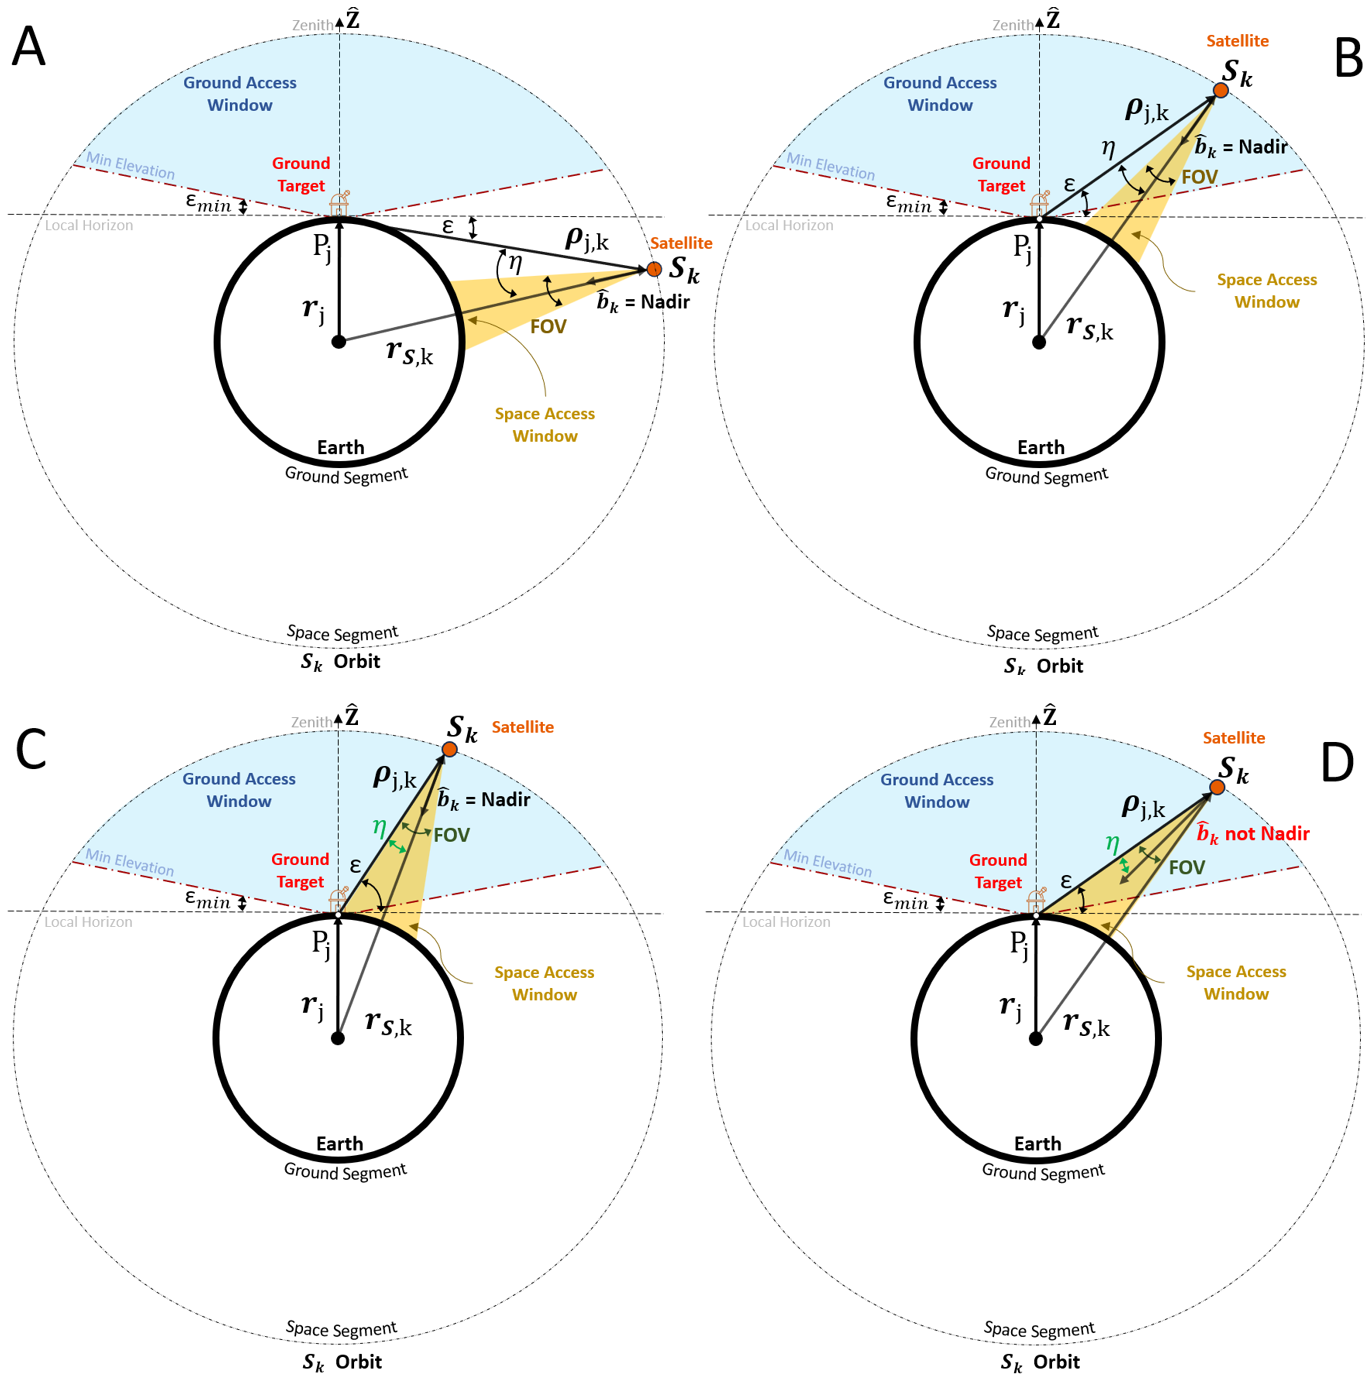
\includegraphics[width=1\linewidth]{images/acess_window_configs.png}
    \caption{\footnotesize{Observational Access Windows configuration. The figure illustrates the interaction between the \textbf{Ground Access Window} (blue cone, defined by tange point $P_j$ and $\epsilon_{min}$) and the \textbf{Space Access Window} (yellow cone, defined by the sensor direction $\hat{b}_k, FOV, $$\eta_{max}$).
    \textbf{(A)} No access: satellite is below the local horizon.
    \textbf{(B)} Ground access, no space access: satellite is above the horizon but with FOV outside $P_j$, or $\eta > FOV$.
    \textbf{(C)} Space \& ground access: satellite see ground $P_j$, ($\epsilon > \epsilon_{min}$) \& ($\eta < FOV$).
    \textbf{(D)} Space \& ground access with pointing out of nadir: $S_k$ uses point mechanism to have valid angular view from $P_j$ $(\theta \leq FOV)$.}}
    \label{fig:access_window_configs}
\end{figure}

\subsection{Ground Segment Access Window ($\mathcal{W}_{ground}$)}
From the perspective of the target $P_j$, $P_j \in \mathcal{F}_{SEZ}$, the satellite $S_k$ must appear within a specific volume of the local sky to ensure a clear signal path. We define the Ground Access Window as the subset in the Topocentric frame $\mathcal{F}_{SEZ}$ where the elevation angle exceeds the minimum operational threshold $\epsilon_{min}$ (imposed by terrain geometric masking and atmospheric attenuation).

Mathematically, this domain is defined by the condition on the relative position vector $\vec{\rho}_{j,k}$ with the spacecraft:
\begin{equation}
    \mathcal{W}_{ground_{j,k}}(t) = \{ \vec{\rho}_{j,k} \in \mathcal{M} \mid \epsilon(\vec{\rho}_{j,k}) \geq \epsilon_{min} \}
\end{equation}
where $\epsilon(\vec{\rho}_{j,k})$ is the elevation calculation defined in the previous section.

\subsection{Space Segment Access Window ($\mathcal{W}_{space}$)}
From the perspective of the satellite $S_k$, the target $P_j$ must lie within the instrument's Field of View (FOV). We define the \textbf{Space Access Window} (or Sensor Cone) based on the instrument's half-cone angle $\eta_{max}$ (FOV limit) relative to the instantaneous boresight vector $\hat{\mathbf{b}}_k(t)$.

The \textbf{Off-Nadir Angle} $\eta_{k,j}$ is defined as the angle between the sensor boresight and the direction to the target (which is $-\vec{\rho}_{j,k}$ in the satellite frame):
\begin{equation}
    \eta_{k,j}(t) = \arccos\left( \frac{-\vec{\rho}_{j,k}(t) \cdot \hat{\mathbf{b}}_{k}(t)}{\| \vec{\rho}_{j,k}(t) \|} \right)
\label{eq:eta}
\end{equation}
The Space Access Window is therefore the volume where this angle satisfies the optical limit:
\begin{equation}
    \mathcal{W}_{space_{j,k}}(t) = \{ \vec{\rho} \in \mathcal{M} \mid \eta(\vec{\rho}_{j,k}, \hat{\mathbf{b}}_k(t)) \leq \eta_{max} \}
\end{equation}
\subsection{Total Visibility Condition}
A valid observation event $E_{obs}$ occurs at time $t$ if and only if the Line-of-Sight vector exists within the intersection of both domains. Formally:
\begin{equation}
    \text{Visible}(t) \iff \vec{\rho}_{j,k}(t) \in \left( \mathcal{W}_{ground_{j,k}}(t) \cap \mathcal{W}_{space_{j,k}}(t) \right)
\end{equation}
This is equivalent to the simultaneous satisfaction of the two scalar inequalities:
\begin{equation}
    \text{Observation Link} \ \mathcal{L}_{j,k}(t) \iff Visible
    \begin{cases} 
        \epsilon_{k,j}(t) \geq \epsilon_{min} =15^{\circ} & \text{(Ground Access Condition)} \\
        \eta_{k,j}(t) \leq \eta_{max} = 65^{\circ} & \text{(Space Access Condition)}
    \end{cases}
    \label{eq:observation_link_condition}
\end{equation}


\section{Principles of Orbital
Mechanics}\label{71-principles-of-orbital-mechanics}

This section introduces the mathematical representation of satellite trajectories and the key gravitational effect that shapes them. The six classical orbital elements describe the size, shape, and orientation of an orbit, while the Earth's equatorial bulge induces predictable secular drifts in the orbital plane. These drifts are not merely perturbations to be corrected --- they are the physical mechanism that makes Repeating Ground Track and Sun-Synchronous orbits possible.

% \begin{itemize}
% \item
%   Explain the six Keplerian orbital elements (a, e, i, Ω, ω, ν) and what they define.
%   \item Introduce the concept of the constellation coverage domain, and how we expect to check this coverage
% \item
%   Discuss key perturbations, focusing on the J2 effect
%   (Earth\textquotesingle s oblateness) and its role in causing nodal
%   precession, which is fundamental to Repeating Ground Track Orbit
%   (RGTO) and Sun-Synchronous Orbits (SSO).
% \item
%   Introduce the concept of a ground track and how it is determined by
%   the orbital period and Earth's rotation.
% \end{itemize}

\subsection{Classical Orbital Elements and Satellite State Vector}
\label{sec:classical_orbital_elements}

To define the trajectory in spacetime of the constellation $\mathcal{C}_{sat}$ (Sec.~\ref{sec:Constellation_observation_form}) within the manifold $\mathcal{M}$, we use the classical Keplerian representation. The state of each satellite $S_k$ is uniquely determined within the inertial reference frame $\mathcal{F}_{J2000}$ by the set of six orbital elements and a reference epoch $t_0$. This is the \textbf{Orbital State Element} vector $\vec{A}_k$ introduced in the constellation formalism, which characterizes the instantaneous geometry of the orbital plane and the position of the spacecraft relative to the Earth's equatorial plane and the reference direction (the First Point of Aries). As illustrated in Fig.~\ref{fig:orbital_elements}, the vector is defined as:
\begin{equation}
    \vec{A}_k = [a, e, i, \Omega, \omega, \nu, t_0]^T
    \label{eq:orbital_state_vector}
\end{equation}
where the orientation of the orbital plane is governed by the Right Ascension of the Ascending Node (RAAN) $\Omega$, the Inclination $i$, and the Argument of Periapsis $\omega$, while the instantaneous position within the orbit is given by the True Anomaly $\nu$. These seven parameters fully determine the satellite's trajectory over the Study Domains $\mathcal{D}$ and constitute the fundamental input to the simulation propagator.

\begin{figure}[H]
    \centering
    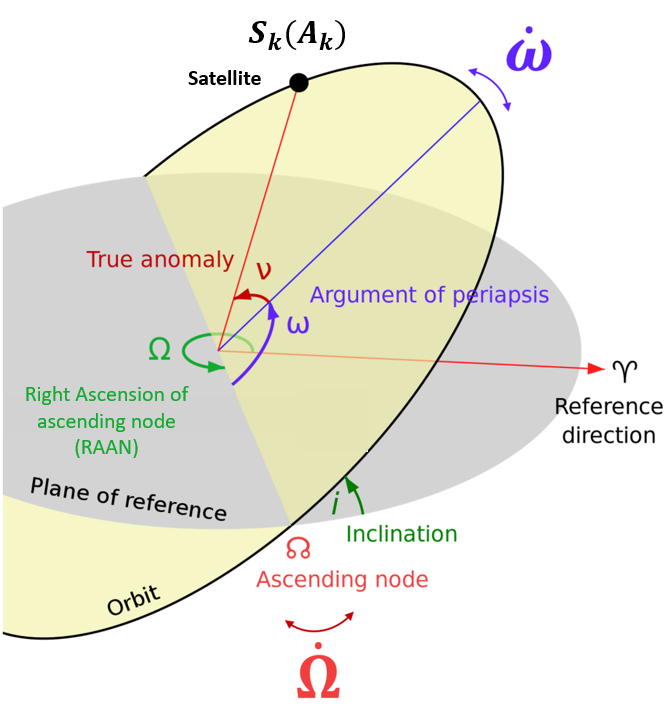
\includegraphics[width=0.5\linewidth]{images/orbital_elements_pertubed_due_J2.png}
    \caption{\footnotesize{Classical Keplerian orbital elements composing $\vec{A}_k$ (Eq.~\ref{eq:orbital_state_vector}): shape ($a$, $e$), plane orientation ($i$, $\Omega$, $\omega$), and in-orbit position ($\nu$) in $\mathcal{F}_{J2000}$. The secular variation (Section \ref{sec:perturbed_orbital_elements}) due to the $J_2$ perturbation: nodal regression rate $\dot{\Omega}$ (Eq.~\ref{eq:dot_Omega}), apidal precession $\dot{\omega}$ (Eq.~\ref{eq:dot_omega} }}
    \label{fig:orbital_elements}
\end{figure}


%===================================================
\section{Gravitational Perturbations and the Geopotential Model}
\label{sec:geopotentialmodel}
%===================================================

Gravitational perturbations caused by Earth's oblateness are a classical problem in astrodynamics.  The non-spherical mass distribution of the Earth---principally the equatorial bulge of approximately 21\,km---gives rise to a gravitational potential that deviates from the idealised Keplerian case $U_0 = \mu/r$.  This potential is conventionally expanded as a series of spherical harmonics characterised by zonal, sectoral, and tesseral coefficients \cite{valladoFundamentalsAstrodynamicsApplications2001}; the complete derivation and the dominant harmonic terms are presented in Appendix~\ref{app:geopotential}.  Among all harmonic coefficients, the second zonal term $J_2 \approx 1.08263 \times 10^{-3}$ exceeds every other coefficient by approximately three orders of magnitude, making it the single most important perturbation for LEO mission design.  The key practical results---the secular drift rates of the ascending node $\dot{\Omega}$, the argument of perigee $\dot{\omega}$, and the mean anomaly $\dot{M}$ induced by $J_2$---are derived below, as they directly determine the Repeating Ground Track Orbit (RGTO) resonance condition used throughout this work.



%===================================================
\subsection{Perturbed Orbital Elements due to \texorpdfstring{$J_2$}{J2}}
\label{sec:perturbed_orbital_elements}
%===================================================

The $J_2$ potential (Appendix~\ref{app:geopotential}) introduces secular rates of change in three of the Keplerian elements within $\vec{A}_k$. Denoting $p = a(1 - e^2)$ as the semi-latus rectum, first-order perturbation theory yields \cite{valladoFundamentalsAstrodynamicsApplications2001}:

\begin{equation}
    \dot{\omega} \;=\; \frac{3}{2}\,J_2
        \left(\frac{R_{\oplus}}{p}\right)^{\!2}
        \sqrt{\frac{\mu_{\oplus}}{a^3}}
        \left[2 - \tfrac{5}{2}\sin^2 i\right],
    \label{eq:dot_omega}
\end{equation}
\begin{equation}
    \dot{\Omega} \;=\; -\frac{3}{2}\,J_2
        \left(\frac{R_{\oplus}}{p}\right)^{\!2}
        \sqrt{\frac{\mu_{\oplus}}{a^3}}
        \cos i,
    \label{eq:dot_Omega}
\end{equation}
\begin{equation}
    \dot{M} \;=\; \sqrt{\frac{\mu_{\oplus}}{a^3}}
        \left[1 - \frac{3}{2}\,J_2
            \left(\frac{R_{\oplus}}{p}\right)^{\!2}
            \sqrt{1 - e^2}
            \left(\tfrac{3}{2}\sin^2 i - 1\right)\right].
    \label{eq:dot_M}
\end{equation}

These secular drifts and their physical consequences for mission design are summarised below. The illustration of this elements are shown in Figure \ref{fig:orbital_elements}.

\paragraph{\textbf{Nodal regression} $\dot{\Omega}$ }
 The ascending node $\Omega$ precesses at a constant rate determined by $a$, $e$, and $i$. For prograde orbits ($i < 90°$) the precession is westward; retrograde orbits ($i > 90°$) produce eastward drift. This rate is the determining factor for both Sun-Synchronous Orbits (SSO) and the resonance condition of Repeating Ground Track (RGT) orbits.
\paragraph{\textbf{Apsidal precession} $\dot{\omega}$}
 The argument of periapsis rotates in the orbital plane. At the \emph{critical inclination} $i \approx 63.4°$ (or $116.6°$), $\dot{\omega} = 0$, making the apoapsis location fixed, a property exploited by Molniya and Tundra orbits and by Flower Constellations using elliptical orbits.
\paragraph{\textbf{Mean-motion correction} $\dot{M}$}
 The effective mean motion departs from the Keplerian value $\sqrt{\mu_\oplus/a^3}$, modifying the satellite's nodal period relative to the nominal two-body case.


These secular rates constitute the astrodynamic foundation for the orbit design methodology developed in the next sections.

%===================================================
\subsection{Geopotential Scope of This Work}
\label{sec:otherharmonics}
%===================================================

Given the dominance of $J_2$ established above (Table~\ref{tab:harmonic_coefficients}), this work adopts two types of force model implementation:

\begin{enumerate}
    \item \textbf{Analytical design}: $J_2$ perturbation alone is for the derivation of the RGTO orbital state (semi-major axis, inclination, and nodal periods). This approximation is valid for defining the satellite's initial state because all other coefficients of the potential perturbation are at least three orders of magnitude smaller. 
    \item \textbf{High-fidelity simulation}: the numerical propagation in GMAT employs a complete force model --- gravitational, third-body, and atmospheric drag;  whose configuration is detailed in the simulation methodology chapter.
\end{enumerate}

\section{Earth Observation Orbits Candidates}
\label{72-earth_orbservation_orbit_candidates}

% """""""improve"
% Orbits are divided in classifications primarly defined by the altitude
% The classcombination of the requirements  of optical quality $GSD=6m/px$, limitsthe altitude 

% \textbf{temporal resolution $\mathbf{{t_{revisit} ≤ 30}}$} minutes and a \textbf{spatial resolution\textbf{ }$\mathbf{{GSD \approx 6 \text{ \textbf{m/pixel}}}}$  }would \textit{significantly improve the accuracy of fire model predictions}\inlineReq{R7}, \inlineReq{R8},

% Repeating Ground-Track Orbits (RGTO) are a class of orbits with specific orbital parameters that ensure the satellite’s ground track over Earth’s surface repeats after a fixed period. This design ensures consistent coverage of areas of interest and predictable revisit times. Furthermore, researchers have \textbf{identified RGTO as the optimal Low Earth Orbit (LEO) type of orbit for minimizing revisit intervals} \autocite{hansonDesigningGoodPartial1990}. Consequently, RGTO serve as the fundamental building blocks for designing LEO \emph{satellite constellations with rapid revisit capabilities}.

% As demonstrated in the coverage chapter, satellites in LEO are the choice of this project for high revisit rate constellation designs, as they provide the \emph{necessary spatial resolution} for wildfire monitoring. Therefore, the following sections will focus \emph{only on LEO circular orbit types}. %TODO: Add chapter reference to coverage chapter

% The following sections establish key physical principles underlying RGTO design, illustrating how these orbits enhance satellite coverage and revisit intervals for Earth observation missions. The RGTO astrodynamics theory presented here is inspired by \citeauthor{leeSatelliteConstellationPattern2020}'s work on Complex Coverage Constellations \autocite{leeSatelliteConstellationPattern2020}.""""


The GSD requirement of $\leq 6$\,m\,px$^{-1}$ constrains the observation altitude to the LEO regime, where the reduced distance delivers the spatial resolution unavailable from MEO or GEO.  Amongst LEO orbit types, the Repeating Ground Track Orbit (RGTO) is selected as the primary orbit family for this mission: it is identified in the literature as the optimal LEO orbit type for minimising revisit intervals over regional targets~\cite{hansonDesigningGoodPartial1990} and its resonance condition can be tuned to the target latitude (Coimbra, $\phi_{\text{lat}} = 40.2^{\circ}$\,N).  The Sun-Synchronous Orbit (SSO), the commercially dominant LEO orbit class for Earth observation, is retained as a comparison baseline; its full astrodynamic development and the quantitative RGTO--SSO comparison are presented in Appendix~\ref{app:sso_orbit}.  The remainder of this chapter develops the astrodynamic foundations of the RGTO.
 

\subsection{Repeating Ground Track Orbit (RGTO) Definition}
\label{72-RGTO_definition}
%-----------------------------------------------------------
% RGTO Orbit Definition
%-----------------------------------------------------------

A Repeating Ground Track Orbit (RGTO) is a class of orbits in which the satellite's sub-satellite ground track closes on itself after a fixed number of orbital revolutions, tracing an identical path over Earth's surface at every successive repeat cycle.  This property ensures consistent, predictable coverage of a target region and deterministic revisit intervals, which are essential for time-critical Earth observation missions.  Hanson~\textit{et al.}\ have formally identified RGTO as the optimal LEO orbit type for minimising revisit intervals over regional targets~\cite{hansonDesigningGoodPartial1990}; consequently, RGTO form the fundamental building block for designing LEO constellations with rapid revisit capability.  The astrodynamic theory developed below is inspired by \citeauthor{lee_satellite_2020}'s treatment of complex coverage constellations \cite{lee_satellite_2020}, a class of flower constellation \cite{mortariFlowerConstellationSet2008}.

\subsubsection{Resonance Condition}
\label{sec:rgto_resonance_condition}

The repeating-track property arises from a \textbf{compatibility} (resonance) condition between two rotating reference frames: the satellite's orbital frame $\mathcal{F}_S$, rotating at the satellite's mean motion $n$, and the Earth-fixed frame $\mathcal{F}_{\oplus}$, rotating at Earth's inertial rate $\omega_{\oplus}$.  Two such frames are compatible if their angular velocities satisfy the rational ratio
\begin{equation}
    N_P \, T_S = N_D \, T_G \,,
    \label{eq:rgto_compatibility}
\end{equation}
where $N_P \in \mathbb{Z}^+$ is the number of complete satellite nodal revolutions, $N_D \in \mathbb{Z}^+$ is the number of Earth rotation periods (nodal days), $T_S$ is the satellite nodal period, and $T_G$ is the Greenwich nodal period.  After $T_r = N_P\,T_S = N_D\,T_G$ the satellite and the Earth-fixed frame return simultaneously to their initial relative geometry, and the ground track closes.

Under the $J_2$ secular perturbation (Sec.~\ref{sec:perturbed_orbital_elements}), the nodal periods depend on the slowly varying orbital elements:
\begin{equation}
    T_S = \frac{2\pi}{\dot{\omega} + \dot{M}}\,, \qquad
    T_G = \frac{2\pi}{\omega_{\oplus} - \dot{\Omega}}\,,
    \label{eq:rgto_nodal_periods}
\end{equation}
where $\dot{\Omega}$, $\dot{\omega}$, and $\dot{M}$ are the $J_2$-driven secular rates of the ascending node, argument of perigee, and mean anomaly, respectively.  The \textbf{period ratio}
\begin{equation}
    \tau \equiv \frac{N_P}{N_D} = \frac{T_G}{T_S}
    = \frac{\dot{\omega} + \dot{M}}{\omega_{\oplus} - \dot{\Omega}}
    \label{eq:rgto_period_ratio}
\end{equation}
uniquely identifies each RGTO family.  OFractions $N_P/N_D$ define distinct ground tracks; for instance $\tau = 10/2$ and $\tau = 5/1$ produce identical repeating patterns.

\subsubsection{RGTO Orbital Element Vector}
\label{sec:rgto_element_vector_def}

Because the semi-major axis $a$ is fully determined by the resonance condition once $\tau$, $e$, and $i$ are fixed,\ $a = a(\tau, e, i)$,  the period ratio $\tau$ replaces $a$ as the independent orbital design parameter.  The \textbf{RGTO orbital element vector} of satellite $S_k$ is therefore defined as
\begin{equation}
    \vec{\mathbf{A}}^{\,\mathrm{RGTO}}{}_{k} = \bigl[\tau,\; e,\; i,\; \Omega,\; \omega,\; \nu,\; t_0\bigr]^{T}\,,
    \label{eq:rgto_element_vector}
\end{equation}
which fully specifies the orbit of $S_k$ within its RGTO family.

\subsubsection{Semi-Major Axis from the Resonance Condition}
\label{sec:rgto_sma_iteration}

Given the resonance integers $N_P$ and $N_D$, the eccentricity $e$, and the inclination $i$, the semi-major axis $a$ is recovered through the iterative scheme of \citeauthor{ulybyshevSatelliteConstellationDesign2008}~\cite{ulybyshevSatelliteConstellationDesign2008}.  An initial Keplerian estimate is obtained from the unperturbed mean motion:
\begin{equation}
    a_0 = \left(\frac{\mu_{\oplus}}{n_0^{2}}\right)^{1/3}, \qquad
    n_0 = \frac{N_P}{N_D}\,\omega_{\oplus}\,,
    \label{eq:rgto_a0_guess}
\end{equation}
where $\omega_{\oplus}$ is Earth's inertial rotation rate.  The $J_2$-corrected value is then refined iteratively:
\begin{equation}
    a_{k+1} = a_0
    \left[1 + \frac{3}{4}\,J_2\!\left(\frac{R_{\oplus}}{a_k}\right)^{\!2}
          \bigl(2 - 3\sin^{2} i\bigr)\right]^{2/3}
    \!\cdot\!
    \left[1 - \frac{3}{4}\,J_2\!\left(\frac{R_{\oplus}}{a_k}\right)^{\!2}
          \!\left(1 + \frac{2\,N_P}{N_D}\cos i - 5\cos^{2} i\right)\right]^{2/3}
    \label{eq:rgto_sma_iteration}
\end{equation}
until convergence $|a_{k+1} - a_k| < \varepsilon$ is reached..  Once $a$ is known, the nodal periods $T_S$ and $T_G$ in Eq.~\eqref{eq:rgto_nodal_periods} and the secular perturbation rates $\dot{\Omega}$, $\dot{\omega}$, $\dot{M}$ follow directly from the expressions derived in Sec.~\ref{sec:perturbed_orbital_elements}.



\subsection{Sun-Synchronous Orbit (SSO)}

A Sun-Synchronous Orbit (SSO) is a near-polar, retrograde orbit ($i > 90^{\circ}$) whose orbital plane precesses eastward at exactly the mean angular rate of the Earth around the Sun, preserving a constant solar-illumination geometry throughout the year.  This constant illumination makes SSOs the predominant choice for optical and multispectral Earth-observation missions and the most commercially accessible LEO orbit class via rideshare launches.  The complete SSO astrodynamic development---including the sun-synchronous condition, the inclination--altitude design equations, and the orbital element vector---is presented in Appendix~\ref{app:sso_orbit}.

With the observation geometry formalised and the astrodynamic foundations in place, the next chapter applies these tools to the mission design. The resonance condition derived here is used to generate the family of Repeating Ground Track Orbit modes tuned to continental Portugal, and a parametric coverage study over that orbit family selects the minimum viable constellation configuration.


